\chapter{软硬兼施} % Introduction chapter suppressed from the table of contents
某次量化根因分析培训里，我跟各现场同学说：“前面我们说可以用鱼骨图分析根本原因，但我不建议在迭代回顾时用它找根因。知道是什么原因吗？请问你是读哪所高校？当时是否自己选的？”

“XX大学。当时是我自己挑选的。”

“现在回想，是否觉得XX大学挺不错？ ”

“是的。”

“如果是自己选择的，都会觉得比其他好。1956年，Brehm 决策影响实验 （详见附件）验证了这心理。所以如果用鱼骨图分析根因，大家都会觉得这只是组长的分析，并非我自己的想法，后面便没有动力执行。”\\


\hypertarget{ux8ba9ux56e2ux961fux6210ux5458ux90fdux79efux6781ux53c2ux4e0e}{%
\subsubsection{让团队成员都积极参与}\label{ux8ba9ux56e2ux961fux6210ux5458ux90fdux79efux6781ux53c2ux4e0e}}

前面的粮食分配实验验证了团队只有兴趣执行自己集体讨论的分析结果，而非听从``专家''意见。所以若要团队做好迭代回顾，取得效果，要注意必须让大家参与，一起分析、讨论，才有动力采取行动。建议使用KJ分析法(详见附件)：每人都有一支水笔+便利贴
，一起找根因，让每人都可以写上自己的意见。如果能让每位团队成员都有充分机会表达意见，不但能集思广益，做到更好的对应方案，也能提升团队后面执行改进方案的积极性。\\
以下经典心理实验解释了为什么KJ分析法，让每位参与者写便利贴这方法，能改善平常大家围着大桌或组长在白板上画鱼骨头等头脑风暴方法的不足。\\

\framebox{%
\begin{minipage}[t]{0.97\columnwidth}\raggedright
想象你在大学读书时被邀请参加某教授的实验。你进入教室，里面已经坐了4位年龄较大的同学，都不认识。

教授投出下图：

%\href{文件:Asch0Screenshot_2022-07-09_161023.jpg}{400px‎}

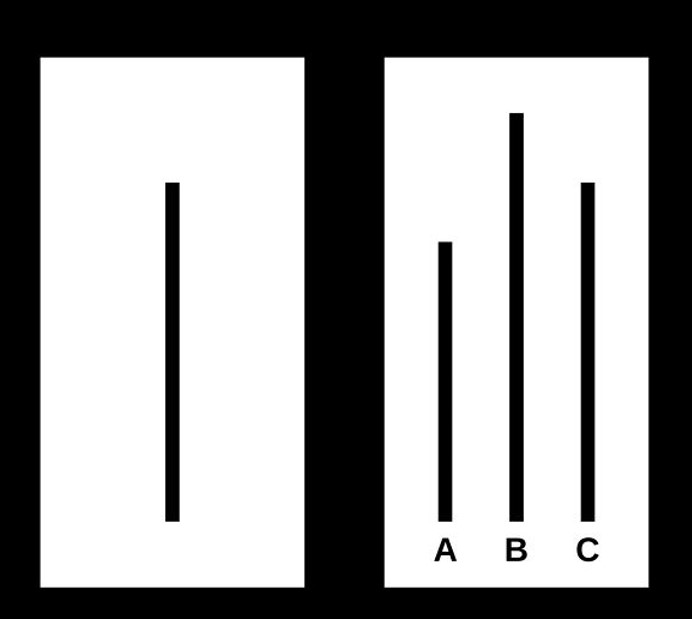
\includegraphics[width=10cm]{Asch0Screenshot_2022-07-09_161023.jpg}

 	
图12-1

然后问：``右面ABC三条线，那条的长度与左面的一条最近？''\\
第一位用了10秒钟仔细考虑后说：``我选B。''\\
第二位考虑后也说：``我选B。''\\
第三、四位也选择B。\\
现在轮到你（第五位），你会选什么？''\\
``C。''\\
``你选C的时候心里怎么想？''\\
``有些疑虑。虽然很清楚正确答案应该是C，但为什么其他4位都选B？会否有些他们懂我不懂的秘密。''\\
``这经典群众压力心理学实验从50年代开始已经重复做了几百次（详见附件），如果在真实实验环境下，如果前面有超过3位都选了错误答案，参加实验者会有30\%错误率，证明
大部分人都会受从众影响。''\strut
\end{minipage}}

做鱼骨图分析时都是某人（通常是组长）拿着水笔自己说自己在墙上的大白板上面画，大部分的原因其实都是组长自己说自己写，其他团队成员都不会主动说自己发现的原因。但如果给每位参与者便利贴和水笔，大家都愿意把想到的写出来。

%\href{文件:!postItMarkerScreenshot_2023-10-27_205505.jpg}{300px}

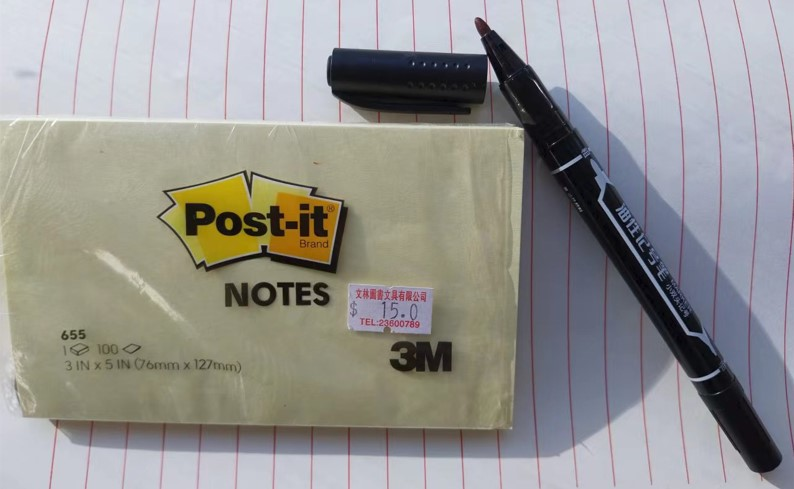
\includegraphics[width=10cm]{!postItMarkerScreenshot_2023-10-27_205505.jpg}

图12-2

\hypertarget{ux56deux987eux6d41ux7a0b}{%
\subsection{回顾流程}\label{ux56deux987eux6d41ux7a0b}}

回顾流程冲刺可以按以下五个步骤进行，确保每位成员都全心投入参与，并通过分析形成行动，达到改进效果：\\
\#设置舞台------ ``热身''，获取对游戏规则共识

\begin{enumerate}
\tightlist
\item
  收集数据（除了收集``硬''数据，如缺陷、工作量、进度偏差等，也要收集``软''数据,如团员感受）
\item
  分析，找出根因
\item
  决定做什么（必须明确下个迭代的具体改进行动到人、任务、时间）
\item
  结束
\end{enumerate}

%\href{文件:178页替换图片.jpg}{500px}

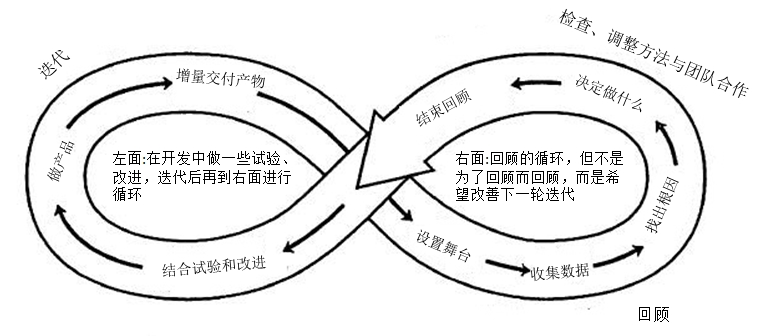
\includegraphics[width=10cm]{178页替换图片.jpg}

图12-3

回顾时，也要想办法避免受到群众压力的影响，导致不能真正挖掘问题的原因。所以在回顾时需要大家放开，以下方法可以减少团队压力，让大家更投入，能畅所欲言：

\begin{itemize}
\tightlist
\item
  回顾开始时（设置舞台），尤其是团队首次在回顾里做集体根因分析，建议用互动游戏，让团队放开顾虑，全心投入讨论（例如附件里``游戏：应与否''）
\end{itemize}

让每位团队成员都有充分机会表达意见，集思广益，得出更好的纠正措施。

\hypertarget{ux56e2ux961fux6240ux6709ux6210ux5458ux53c2ux4e0e}{%
\subsubsection{团队所有成员参与}\label{ux56e2ux961fux6240ux6709ux6210ux5458ux53c2ux4e0e}}

整个团队参与分析，全面看问题。例如如果只是从测试人员的角度，他可能以为缺陷都是来自开发；需求分析人员（或产品经理）会觉得自己做得很好，因需求评审里没有什么问题被发现。但如果团队所有成员聚在一起（包括项目经理、需求、设计、编码、测试），把所有的缺陷列出来，让团队所有岗位一起分析，才可以全局看问题，才可能发现不少问题是因为需求没有明确，导致后面做出来的功能并不是客户要的。后面可扩大参与回顾的干系人，例如客户代表，可以更全面分析。\\

\hypertarget{ux6570ux636eux51c6ux5907}{%
\subsubsection{数据准备}\label{ux6570ux636eux51c6ux5907}}

有数据才有管理，但软件开发与工厂不同，很多数据必须依靠员工提供，

例如，某活动所花的工时，必须靠个人记录（具体步骤可参考``个人量化管理''：个人记录每天工时）。

但记录数据要花精力，如果不了解收集的数据，后面有什么用途，便难以维持不断收集数据的习惯。如果当大家都清楚到迭代回顾时会一起分析团队数据，并制订改进措施，就有动力继续迭代里统计数据。\\
也解释了为什么依赖公司级数据分析专员收集并分析团队数据，因通常几个月后才收到数据分析的反馈，公司难以收到真实的数值。\\

\hypertarget{ux5185ux90e8ux6559ux7ec3ux5982ux4f55ux505aux597dux73b0ux573aux8f85ux5bfc}{%
\subsection{内部教练如何做好现场辅导}\label{ux5185ux90e8ux6559ux7ec3ux5982ux4f55ux505aux597dux73b0ux573aux8f85ux5bfc}}

培训后过了6周，质量经理电话联系我。\\
质量经理：我们计划下周三与项目组进行迭代回顾。该团队有7到8人，两周前曾与另一团队使用便利贴进行了根因分析，确实听到了更多不同的声音。应该如何准备，才能让团队放开并有效地做好根因分析？\\
我：如果只有缺陷数量和工作量等``硬''数据，但缺乏如团队成员的感受、积极性、主动性等与人性相关的``软''数据，也难以真正分析出能够避免同类问题再次发生的根本原因。例如，在冲刺回顾时可以用时间表（Timeline）让大家回忆过去四周的经历，并用颜色点（Color
Code
Dots）让每位成员标记每个事件的感受，这是一种收集软数据的方法，详见附件：敏捷回顾互动练习。\\
要做好回顾，准备工作至关重要。例如需要准备大白纸，并确保有足够的空间。如果团队成员围坐在一个大桌子旁讨论，效果往往不佳。相反，我们在墙上贴上大白纸，并提供便利贴和大号、小号水笔等，当每个人都有自己的一支笔时，团队成员会更加投入。他们会走动、讨论、写字、画图，并不断交换位置、互相帮助，这样能更好地体现团队精神。因此，辅导的重点不是在各种技巧上，不是教他们每一步怎么做，只需提醒时间（时间的管理很重要。每次进行小组练习时，我都会用电脑投屏显示剩余时间（分钟），让团队即时掌握剩余的时间）。先定好目标，让团队自主发挥与讨论，效果会更好。只要他们清楚需要做什么，大部分团队都能自行分工，比如有些人负责画帕累托图，有些人做总体根因分析。\\
质量经理：你的意思是减少干预，尽量让团队自主思考。但因未做过，可否再举些例子？\\
我：正确。不如我反过来，建议你应该避免说什么：

\begin{enumerate}
\tightlist
\item
  其实你们团队和我见到的其他团队相比好或者差（因这都是个人观点、感觉，非事实）
\item
  本来只需要你们画帕累托图和鱼骨图，为什么你们还画了个脑图
\item
  你们都已经讨论了很多细节，要立马赶紧时间做最后总结
\item
  你们讨论好像都只是针对机场闸口的问题，是否应该也考虑其它
\end{enumerate}

为什么要鼓励团队表达不同意见？\\
团队要改进，首先要确保成员充分理解彼此的差异。经过充分讨论后，团队成员找到共同点，才有机会一起改进。\\
如果大家在回顾时能够开放讨论，充分表达各自具体的看法，就能让大家看到全貌和问题的真正情况。\\
因此，内部教练应鼓励多样化的声音。心理学家 Asch 在 1951
年的从众实验中证明，只要有一个人率先提出异议，其他人也会陆续表达自己的意见。因此，内部顾问应确保每个人都有发声的机会。意见越多样化，大家越能了解真正的问题，找到大家认可的改进方案（详见附件：功能性分组帮助团队成长实例）。\\
例如，如果发现团队在大型会议上因人数众多而不愿发言，可以考虑分成小组讨论，这通常会更有效。\\
对于一些``慢热''的团队，需要给予他们更多时间，不要急于打破沉默。等一等，一旦有人开始发言，接下来的讨论就顺利了。\\

\hypertarget{ux56e2ux961fux8fedux4ee3ux56deux987eux6839ux56e0ux5206ux6790ux5e38ux89c1ux95eeux9898}{%
\subsection{团队迭代回顾根因分析常见问题}\label{ux56e2ux961fux8fedux4ee3ux56deux987eux6839ux56e0ux5206ux6790ux5e38ux89c1ux95eeux9898}}

\begin{enumerate}
\tightlist
\item
  没有利用缺陷数据做帕累托图分析，不清楚应针对哪一类，不清楚哪一类问题最多，导致根因分析讨论没有针对性。有些缺陷分类没有定义好、不明确或同一缺陷归到几个类别，导致分析结果没有参考作用
\item
  不清楚什么是根因，只找到表面看到的现象，例如人经验不足，对技术不熟悉，对业务不熟悉等。没有抓到系统的根本问题
\item
  没有量化目标，只有定性的根因分析，下轮迭代难以判断效果能否达到
\item
  回顾时间不够（足够的时间，最少3小时）
\end{enumerate}

以上前3点可以利用培训，加强上章讲过的根因分析方法。\\
最后一点需要领导理解如果想要有效，必须收集数据，并让团员投入讨论。

\framebox{%
\begin{minipage}[t]{0.97\columnwidth}\raggedright
研发总监：已经做了很多年过程量化考核，起初能给团队带来活力，因为至少比以前好，有路径可以量化他们，员工觉得做有所值，公司也看得见。前几年执行得很好，产出和上线频率比过去好很多。但是现在感觉逐渐拉不出差距来，因为大家都非常熟悉这套游戏规则。\\ 我：理解，比如现在你们团队开始做迭代回顾，团队一起分析根因，持续改善。您觉得效果如何？\\ 研发总监：挺好，但是还是感觉他们开回顾会，耗时太长了，每次都要2小时以上。\\ 我：因需要团队收集数据、分析、讨论下迭代措施，所以通常要3小时，熟练后会快一点，底线是改进的节省应大于回顾的投入。\\ 高层的支持是任何改进的重要成功要素。所以首先要让管理者赞同迭代回顾能为公司带来回报（省钱)，可以节省的成本（工作量）大于回顾的人力投入；也要让他理解任何改变都有个混沌的过渡期，要经过几轮回顾后，团队才能自己持续改善。

\strut
\end{minipage}}


\framebox{%
\begin{minipage}[t]{0.97\columnwidth}\raggedright
如果回顾只能1个或1个半小时的话,就不够时间让团队针对缺陷分组分类、画帕累托图做分析，没有根据实际数据分析根因，也影响到团队没有动力在后面迭代花精力去收集数据。例如缺陷返工数据一直都非常难获取得到的，也需要在迭代根因分析时给团队时间讨论统计，所以通常完整的迭代根因分析回顾不会小于3小时。要做好这块如果有内部教练可以更好控制整个回顾的节奏。不会在某一个环节耽误太多时间，也不会太长，也确保团队人员都全程投入讨论。


\strut
\end{minipage}}

所以要团队做好迭代回顾，内部教练不仅仅教大家各种``硬''技巧，也要考虑影响大家的心理，必须让每位成员都积极参与，才有动力执行和以后继续积极参与。
如果只是组长一言堂，反而会妨碍团队成员的动力。
但是只依赖大家的经验和感觉，识别根本原因也不科学，所以也必须有数据支撑（硬的内容）。\\
当然也需要高层支撑------提供资源和时间，如高层觉得整个团队花半天来做回顾太浪费资源，也无法推行。\\
下一章我们会分享一些团队对回顾的误解和常见问题。

\hypertarget{ux9644ux4ef6}{%
\section{附件}\label{ux9644ux4ef6}}

\hypertarget{asch-1951-ux7fa4ux4f17ux538bux529bux5b9eux9a8c}{%
\subsection{Asch 1951
群众压力实验}\label{asch-1951-ux7fa4ux4f17ux538bux529bux5b9eux9a8c}}

实验设计：\textbf{随机邀请几位志愿者（包括你）参加，实验之前与（除了你以外）所有人预先说好，都选A，并且要假装成经过深思熟虑。实验时，你是最后一位作答。}

结果：

\begin{itemize}
\tightlist
\item
  有群众压力时，大概\textbf{37\%}会从众选择错误答案(虽然不同人有差异，但总体只有\textbf{25\%}能坚持自己的正确答案)
\item
  个人自己作答，接近100\%选对，错误率\textbf{少于1\%}
\end{itemize}

影响因素:

\begin{itemize}
\tightlist
\item
  前面选择错误答案的人数越多，错误率越高:
\end{itemize}

\begin{enumerate}
\tightlist
\item
  一位：接近0\%答错
\item
  两位：大概14\%
\item
  三位: 32\%（详见下图）
\end{enumerate}

%\href{文件:Asch3Screenshot_2022-07-08_201341.1.png}{500px‎}

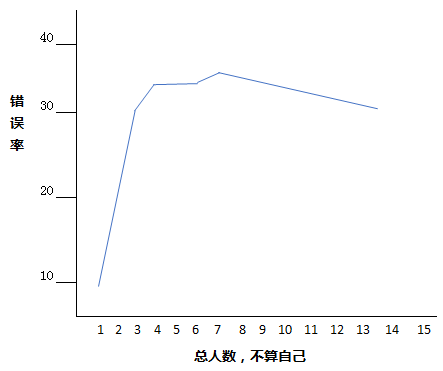
\includegraphics[width=10cm]{Asch3Screenshot_2022-07-08_2013411.png}

 	
图12-4

\begin{itemize}
\tightlist
\item
  如果前面有一位``战友''选了正确答案，你的错误率就显著降低（大约原本水平的1/4，看下图黄线），并让你感到与他更亲切
\end{itemize}

%\href{文件:Asch4Screenshot_2022-07-08_201502.1.png}{500px‎}

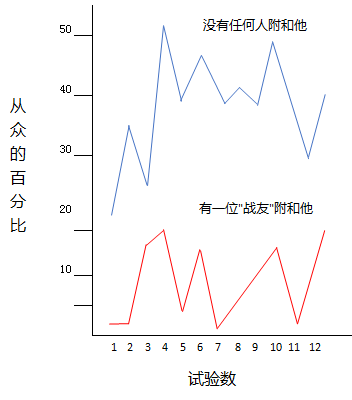
\includegraphics[width=10cm]{Asch4Screenshot_2022-07-08_2015021.png}

图12-5

\begin{itemize}
\tightlist
\item
  尴尬场景(例如迟到)，你的错误率会更高

  \begin{itemize}
  \tightlist
  \item
    实际你没有晚到，只是让你觉得确实迟到了，觉得尴尬
  \end{itemize}
\item
  如果不是要你说出答案，而是让你把答案写在纸上，错误率会降低1/3
\end{itemize}

\hypertarget{brehm-1956-ux51b3ux7b56ux5f71ux54cdux5b9eux9a8c}{%
\subsection{Brehm 1956
决策影响实验}\label{brehm-1956-ux51b3ux7b56ux5f71ux54cdux5b9eux9a8c}}

\textbf{实验设计}：

\begin{enumerate}
\tightlist
\item
  提供10多种不同礼物，包括台灯、多士炉、挂钟、收音机等
\item
  请你按自己喜好对礼物排序。例如最喜欢的选一，如果同样喜欢两件礼物，可以不分高低，写同一个数字
\item
  但当你马上要离开时，让你从两件同样喜好的礼物挑选其中一件，让你拿走
\item
  在你最终离开之前，请你再对所有礼物按喜好排序
\end{enumerate}

\textbf{结果}：

\begin{itemize}
\tightlist
\item
  绝大部分人都会抬高自己选择拿走的那一件礼物排序，调低非选择的那件礼物排序
\item
  但如果不是自己选择，而是由老师选好给你，你后面的礼物排序就没有变化
\end{itemize}

\textbf{结论}：

\begin{itemize}
\tightlist
\item
  人都会觉得自己的选择比较好
\item
  例如选大学、选汽车、选伴侣。如果是由你自己决定选择（非被安排），你会不会都会觉得自己的选择较好
\end{itemize}

\hypertarget{kjux5206ux6790ux65b9ux6cd5ux6b65ux9aa4}{%
\subsection{KJ分析方法步骤}\label{kjux5206ux6790ux65b9ux6cd5ux6b65ux9aa4}}

\hypertarget{ux8ba9ux56e2ux961fux4e86ux89e3ux5927ux5bb6ux7684ux4e8bux5b9eux4e00ux8d77ux5206ux6790ux6839ux56e0ux4e00ux8d77ux505aux5206ux6790ux62a5ux544a}{%
\subsubsection{让团队了解大家的事实，一起分析根因，一起做分析报告}\label{ux8ba9ux56e2ux961fux4e86ux89e3ux5927ux5bb6ux7684ux4e8bux5b9eux4e00ux8d77ux5206ux6790ux6839ux56e0ux4e00ux8d77ux505aux5206ux6790ux62a5ux544a}}

\begin{itemize}
\tightlist
\item
  大家都对着墙上的大白纸
\end{itemize}

%\href{文件:KJ1.jpg}{400px}


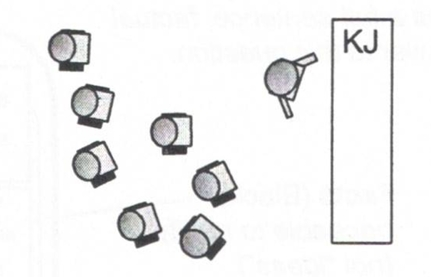
\includegraphics[width=10cm]{KJ1.jpg}

图12-6

\begin{itemize}
\tightlist
\item
  每人依据主题写``事实''并写在便利贴上，贴到大白纸上
\end{itemize}

%\href{文件:KJ2.jpg}{600px}

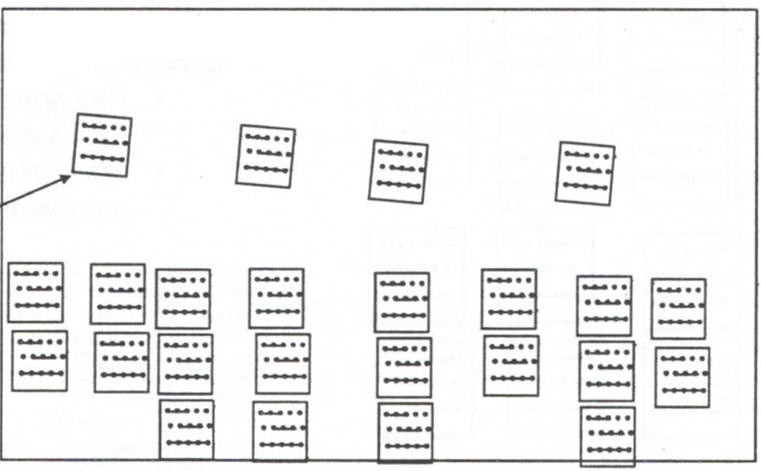
\includegraphics[width=10cm]{KJ2.jpg}

图12-7

\begin{itemize}
\tightlist
\item
  轮流移动上面的便利贴，经过1\textasciitilde{}2轮后，逐渐看到归类
\item
  大家一起挖掘隐藏在低层次事实中的更通用的重点
\end{itemize}

%\href{文件:KJ3.jpg}{600px}

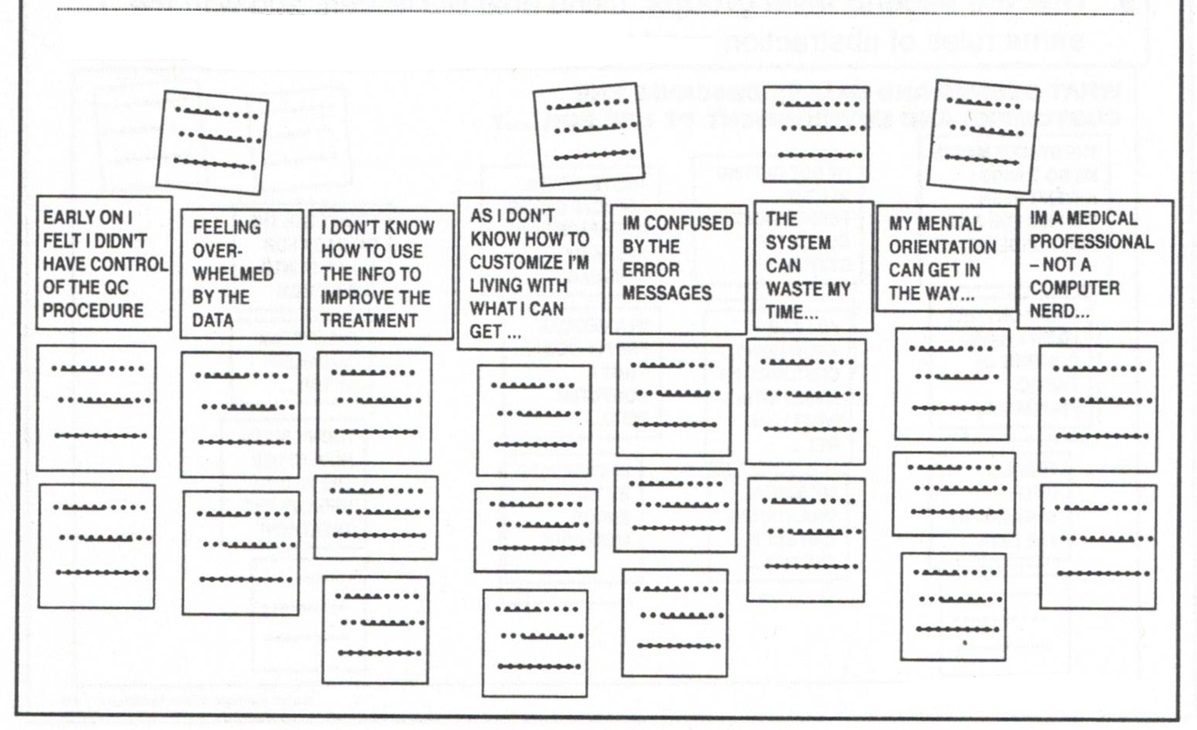
\includegraphics[width=10cm]{KJ3.jpg}

图12-8

\emph{一种头脑风暴方法，每人把自己想法写在便利贴上，一起轮流把所有便利贴排放分组}

\begin{enumerate}
\tightlist
\item
  把主题以问题形式写在大白纸的头顶
\item
  把相关的事实写在便利贴上面，用黑色
\item
  搜集相关的事实，如果是一组人的话，分散到不同人手上
\item
  （团队）查看描述是否不清楚，是否要整理
\item
  每人轮流把相关的便利贴组合在一起
\item
  当每人都已经调整过便利贴组合后，一起把每一组便利贴加上一个题目，用红色标识
\item
  红色的标题下包含相关事实的内容
\item
  把相关的红色题目（最好不超过3个）组合在一起
\item
  给这大组一个题目------蓝色
\item
  在题目下放上相关的红色小组
\item
  把蓝色的题目和剩下红色的小组或单独没有分类的便利贴都在墙上放好，也可以用一些箭头描述它们的因果关系
\end{enumerate}

%\href{文件:206页替换图片.jpg}{600px}

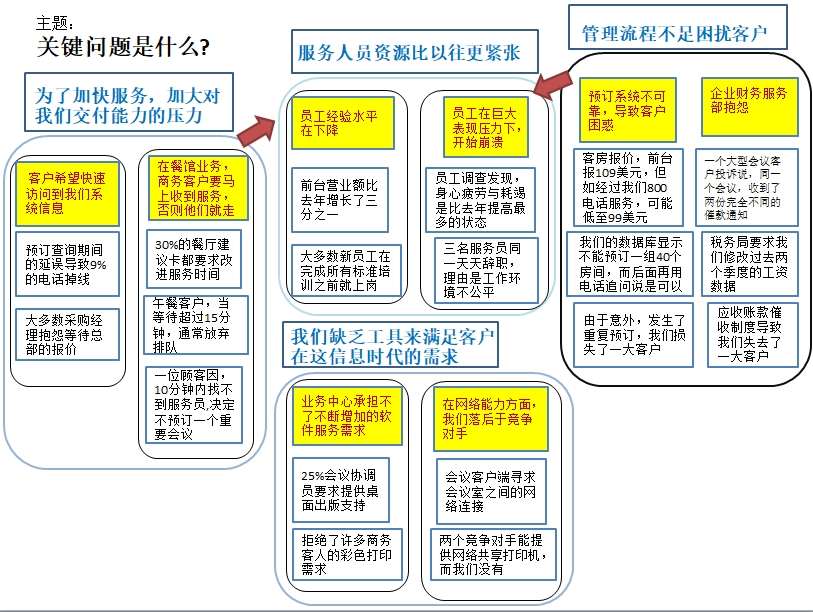
\includegraphics[width=10cm]{206页替换图片.jpg}

图12-9

利用便利贴做KJ分析让大家都充分参与，不仅仅适用于迭代回顾。我每次培训，如果有时间，尽量最后腾出1个小时，让大家归纳刚刚学过的东西，按自己日常工作不足可以改善之处进行分析根因，并制定改进计划。本来上课时无精打采的学生都会立马精神过来，积极参与讨论。后面有些同学在填培训反馈表时，
还建议应再多分配时间给学生互动讨论，减少讲课和个人做练习的时间。

\hypertarget{ux6e38ux620fux5e94ux4e0eux5426}{%
\subsection{游戏:应与否}\label{ux6e38ux620fux5e94ux4e0eux5426}}

在迭代回顾中使用。

\hypertarget{ux76eeux7684}{%
\subsubsection{目的}\label{ux76eeux7684}}

帮助建立有效沟通的思维模式。帮助参与者抛开指责和判断，以及对指责和判断的恐惧。

\hypertarget{ux6240ux9700ux7684ux65f6ux95f4}{%
\subsubsection{所需的时间}\label{ux6240ux9700ux7684ux65f6ux95f4}}

8 \textasciitilde{} 12分钟，取决于小组的大小。

\hypertarget{ux63cfux8ff0}{%
\subsubsection{描述}\label{ux63cfux8ff0}}

在描述这些模式之后，参与者讨论这些沟通模式的意义。

\hypertarget{ux6b65ux9aa4}{%
\subsubsection{步骤}\label{ux6b65ux9aa4}}

\begin{enumerate}
\tightlist
\item
  将注意力集中在``应与否''(见下图)，并简要阅读
\item
  组成小组，每组不超过4人。要求每组用一对词来定义和描述，有4对以上的词组。如果有多个组有相同的词组也可以
\item
  让每个小组讨论他们的2个单词的意思和它们所代表的行为，让他们描述各自对团队和回顾的影响
\item
  每个小组向整个小组汇报他们的讨论情况
\item
  询问大家是否愿意使用左面的方式
\end{enumerate}

%\href{文件:_游戏1应与否1.png}{500px}

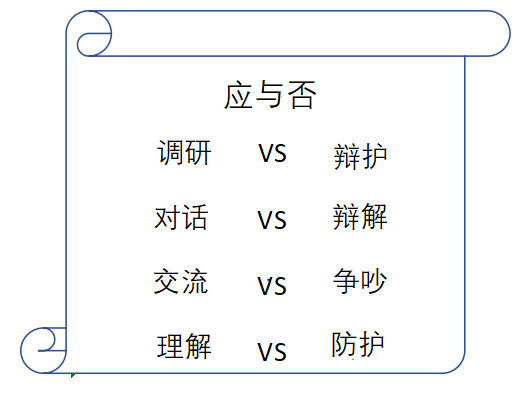
\includegraphics[width=10cm]{游戏1应与否1.png}

图12-10

\hypertarget{ux7528ux89d2ux8272ux626eux6f14ux4e3aux505aux597dux56deux987eux6253ux57faux7840}{%
\subsubsection{用角色扮演为做好回顾打基础}\label{ux7528ux89d2ux8272ux626eux6f14ux4e3aux505aux597dux56deux987eux6253ux57faux7840}}

首次现场培训时，我都会要求角色扮演：学员用各种角色扮演什么是吵架、什么是交流，让观众和表演者更能感受到量化回顾先要有对事不对人的心态。

除了能提高学员的参与度，也能让大家能更好理解左面与右面的区分。

\hypertarget{ux529fux80fdux6027ux5206ux7ec4ux5e2eux52a9ux56e2ux961fux6210ux957fux5b9eux4f8b}{%
\subsection{功能性分组帮助团队成长实例}\label{ux529fux80fdux6027ux5206ux7ec4ux5e2eux52a9ux56e2ux961fux6210ux957fux5b9eux4f8b}}

系统，包括团队、公司的成长都依靠不断集合内部的差异，如果完全不能接受不同意见，就无法进步。基于心理学家Yvonne
Agazarian系统中心理论(Systems Centered
Theory)，团队必须先从传统（按岗位、功能）分组(Stereotype Subgroup)
变为功能性分组(Functional Subgroup)，才能成长。\\
要让大家觉得有共同点，基于这基础才可以听从不同意见。


\framebox{%
\begin{minipage}[t]{0.97\columnwidth}\raggedright
场景实例\\
 团队讨论如何完善社区里面的教育，大家讨论个人的希望。\\
 A：好像我们大家的想法都很类似。\\
 内部教练：可否举个例子？\\
 B：我们都想为自己和我们后代有个终身不断学习的机会。\\
 C：好像我们都没有人提过大学，不知道为什么。\\
 D：但很多人负担不起大学学费。\\
 E：我觉得每个人只要想受到教育，都能做到，我就是靠自身努力。最后完成大学教育。\\
 F：（开始跟D形成小组）是的，但教育确实越来越昂贵，
我估计我们当中不少人负担不起那些美国东岸名校的昂贵学费。\\
 G：（有成见，觉得那些不能完成大学教育的都是没有动力，没有上进心）我还是觉得任何人，只要有动力都能做到。\\
 如果没有人附和E的观点，就可能变成他的个人独角戏。后面有两个可能的发展场景：\\
 场景一
C 附和了E
的观点。\\
 C：我的经历确实和E说的类似，辛辛苦苦最终完成了大学教育，但确实很艰苦。
如果我当时没有舅舅的支持，肯定完成不了。\\
 场景二 没有人附和
E
的说法。\\
 内部教练：有没有其他人也有经过自己努力完成大学教育的经历？\\
 （注意：内部教练千万不能说：``有没有人赞同，人只要有动力都能进大学？''因为这只是个人观点，并非事实。）\\
 A：我确实也完成了大学教育了，但也经历了很多困难。\\
G：我读了一年，因为再得不到奖学金，没有办法，只能退学。\\
 到了这个点，整个分组就比较复杂，虽然生成了新小组，E得到一些回应，但也有些人提出不同的经验，需要有说法把新小组归纳。\\
接下来，\\
 C：我看来这个很简单，有些人能完成大学教育。有些人虽然很希望完成，最终还是完成不了，但不是所有人都想或者必须完成大学教育。所以我们的改进任务应该是帮助所有人学到他希望学习的东西。\\
 有了以上C的说法，整个团队就可以进一步成长。

\strut
\end{minipage}}

\hypertarget{ux654fux6377ux56deux987eux4e92ux52a8ux7ec3ux4e601ux65f6ux95f4ux8868-timeline}{%
\subsection{敏捷回顾互动练习1:时间表
(Timeline)}\label{ux654fux6377ux56deux987eux4e92ux52a8ux7ec3ux4e601ux65f6ux95f4ux8868-timeline}}

在较长的迭代、发布或项目回顾中使用此方法收集数据。

\hypertarget{ux76eeux7684-1}{%
\subsubsection{目的}\label{ux76eeux7684-1}}

促进大家记忆，从多个角度回看之前的工作。大家一起回看谁在什么时候做了什么工作，与当初的假设对比。看是否有什么规律？或者生产水平有没有变化？用来表达事实和每人的感受。

\hypertarget{ux6240ux9700ux7684ux65f6ux95f4-1}{%
\subsubsection{所需的时间}\label{ux6240ux9700ux7684ux65f6ux95f4-1}}

30到90分钟，这取决于团队的规模和迭代周期长短。

\hypertarget{ux63cfux8ff0-1}{%
\subsubsection{描述}\label{ux63cfux8ff0-1}}

小组成员写卡片来标示那些很有印象、特别有意义或其他重要事件，然后按时间顺序贴在时间表
(Timeline)上。教练鼓励团队讨论事件，以了解已发生的事实和感受。

变化：功能性泳道 Functional Swim Lanes \\
沿时间轴的背景线纵向绘制行(假设你不打算直接在墙上张贴卡片，然后使用丝带或胶带划分行)。为每个部门或功能做一行。每组只会把他们的卡片放在自己组的泳道里。

%\href{文件:泳道图1.jpg}{650px}

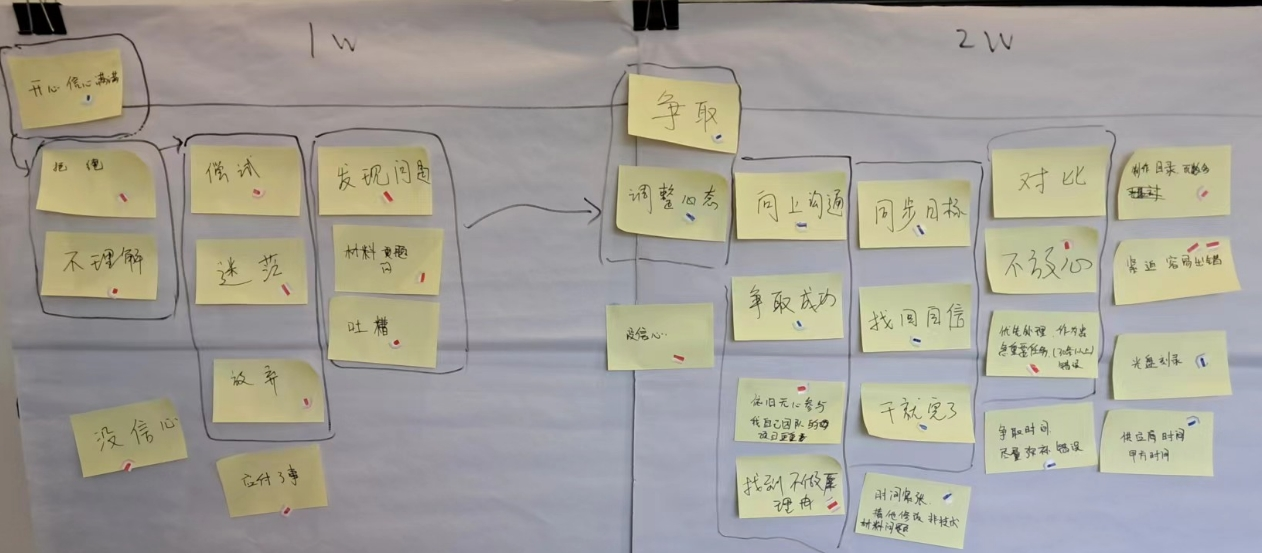
\includegraphics[width=10cm]{泳道图1.jpg}

图12-11

\hypertarget{ux654fux6377ux56deux987eux4e92ux52a8ux7ec3ux4e602-ux989cux8272ux70b9-color-code-dots}{%
\subsection{敏捷回顾互动练习2: 颜色点 (Color Code
Dots)}\label{ux654fux6377ux56deux987eux4e92ux52a8ux7ec3ux4e602-ux989cux8272ux70b9-color-code-dots}}

与时间表(Timeline)练习结合使用，在更长的迭代回顾中收集团员的感受。

\hypertarget{ux76eeux7684-2}{%
\subsubsection{目的}\label{ux76eeux7684-2}}

展示团队成员对经历事件的感受。

\hypertarget{ux6240ux9700ux7684ux65f6ux95f4-2}{%
\subsubsection{所需的时间}\label{ux6240ux9700ux7684ux65f6ux95f4-2}}

5至20分钟。

\hypertarget{ux63cfux8ff0-2}{%
\subsubsection{描述}\label{ux63cfux8ff0-2}}

团队成员使用颜色点来表示在时间轴上事件的心情高低。
当所有的事件都已经展示在时间轴上，团队也已经回顾后，每人使用颜色点来显示他们的情绪是高还是低(见图)。

\begin{enumerate}
\tightlist
\item
  ``我们已经一起看了事实，让我们也看看大家工作时的心情，状态''。
  作为开始之前说，让大家理解游戏目的
\item
  给每个人提供两种颜色的点。每人从7到10个点开始，如后面不够用，可提供更多。解释哪种颜色代表情绪高，哪种颜色代表情绪低
\item
  让每个人都用点来表示哪里情绪高，哪里停滞、衰弱或低潮
\end{enumerate}

%\href{文件:颜色点1.jpg}{300px}


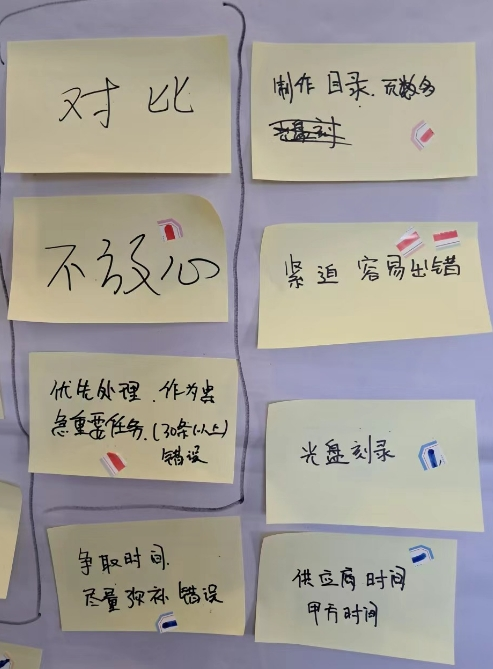
\includegraphics[width=10cm]{颜色点1.jpg}

图12-12
